\chapter{Il Mondo dei Sogni} \label{cap:mondo-dei-sogni}

Ogni persona ha almeno un sogno ogni notte.
Alcuni sogni vengono dimenticati immediatamente al risveglio, altri vengono ricordati per mesi o addirittura anni.
I loro contenuti vanno dal curiosamente bizzarro all'iperrealistico, dall'incredibilmente bello all'indicibilmente
terrificante.
Per questi motivi, l'umanità è stata affascinata dal mondo dei sogni fin dagli albori della storia documentata.
Nel campo scientifico, tre principali approcci si sono differenziati tra loro nello studio dei sogni, essi sono
l'approccio psicoanalitico~\cite{Ruby2011ExperimentalRO}, neurofisiologico~\cite{Akhtar2022} e psicologico~\cite{Schredl2005}.

Le esperienze che costituiscono il sogno emergono casualmente dal cervello, oppure affiorano in base a determinati
parametri?
I sogni hanno un significato?
Qual è o quali sono le funzioni del sognare?
Lo scopo della psicoanalisi è quello di fornire ipotesi per rispondere a queste domande.

L'approccio neuropsicologico è invece interessato alla fenomenologia dei sogni e alla sua relazione con l'attività
cerebrale, concentrandosi sul come le informazioni vengano elaborate durante il sonno e sul ruolo delle varie regioni
cerebrali specializzate rispetto all'esperienza onirica.

Infine, l'approccio psicologico si concentra su una ricerca orientata da aree di interesse quali
la natura e la descrizione dei sogni, i fattori che influenzano il contenuto dei sogni e l'influenza dei sogni sulla
vita diurna.

In questo breve capitolo si cercherà di dare una concisa panoramica generale sul mondo dei sogni, integrando le diverse
prospettive sopra citate e attingendo da informazioni provenienti da svariati studi scientifici che hanno contribuito
a descrivere lo stato dell'arte attuale in questo campo.


\section{Perché sogniamo?}
Sebbene le scienze mediche abbiano fatto enormi progressi negli ultimi sessantacinque nell'intento di comprendere il
sonno e le relative attività cerebrali, medici e scienziati non sono ancora riusciti a spiegare con esattezza la
natura e le ragioni del sogno.
Questo è il motivo per cui i sogni sono ancora ritenuti un campo di ricerca misterioso ed affascinante: non esiste
tutt'ora una loro spiegazione univoca e condivisa.

Prima di tentare di comprendere i sogni, però, è fondamentale che si conoscano i meccanismi del sonno.
Il sonno non è uniforme.
Durante la notte, la totalità del periodo di sonno può essere scomposta in diversi cicli, ciascuno dei quali è
composto da una sequenza di quattro fasi principali.
In una notte tipica, una persona attraversa da quattro a sei cicli di sonno.
Non tutti i cicli di sonno hanno la stessa durata, tuttavia, essa si attesta attorno ad una media di 90 minuti per
ciascuno.

\begin{figure}[t]
    \centering
    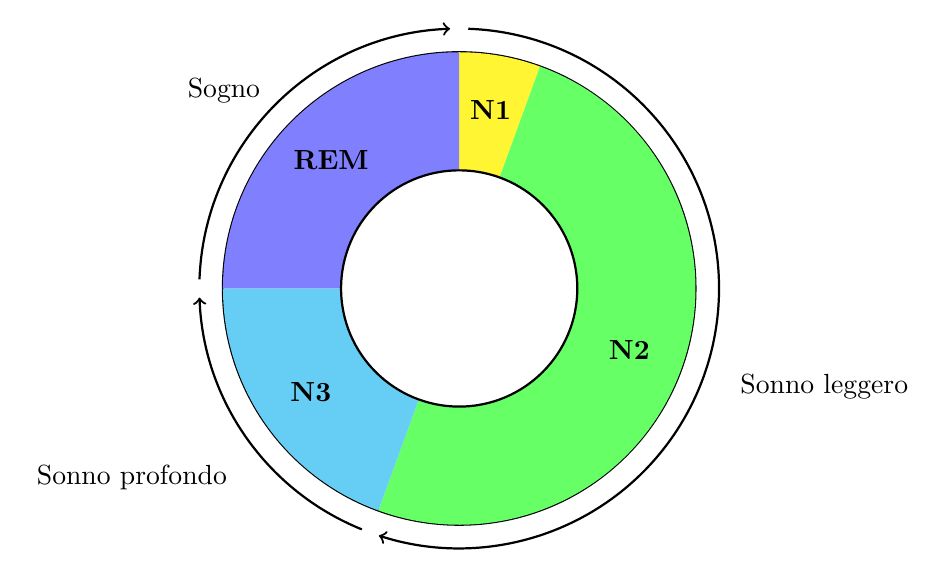
\begin{tikzpicture}

% Circle base
\draw[thick] (0,0) circle (3cm);

% Sectors
% Sectors
\fill[yellow!80] (0,0) -- (90:3cm) arc[start angle=90, end angle=70, radius=3cm] -- cycle;
\fill[green!60] (0,0) -- (70:3cm) arc[start angle=70, end angle=-110, radius=3cm] -- cycle;
\fill[cyan!60] (0,0) -- (250:3cm) arc[start angle=250, end angle=180, radius=3cm] -- cycle;
\fill[blue!50] (0,0) -- (180:3cm) arc[start angle=180, end angle=90, radius=3cm] -- cycle;

% Inner circle
\draw[thick, fill=white] (0,0) circle (1.5cm);

% Text
%\node at (0,0) {\text{Ciclo del Sonno}};
\node at (80:2.3cm) {\textbf{N1}};
\node at (340:2.3cm) {\textbf{N2}};
\node at (215:2.3cm) {\textbf{N3}};
\node at (135:2.3cm) {\textbf{REM}};

% Arrows and labels
\draw[->, thick] (88:3.3cm) arc[start angle=88, end angle=-108, radius=3.3cm];
\node at (345:4.8cm) {Sonno leggero};

\draw[->, thick] (248:3.3cm) arc[start angle=248, end angle=182, radius=3.3cm];
\node at (210:4.8cm) {Sonno profondo};

\draw[->, thick] (178:3.3cm) arc[start angle=178, end angle=92, radius=3.3cm];
\node at (140:3.9cm) {Sogno};

\end{tikzpicture}
    \vspace{-10pt}
    \caption{Il ciclo del sonno}
    \label{fig:sleep-cycle}
\end{figure}

Le quattro fasi principali di ogni ciclo sono N1, N2, N3 e REM, acronimo di \textit{Rapid Eye Movement}.
La fase N1 è quella che consiste del sonno più leggero.
Infatti durante questa fase, una persona può essere svegliata facilmente.
Durante la fase N2, le attività neuronali iniziano a rallentare, preparando il nostro corpo per il sonno
profondo.
La fase N3 è conosciuta come sonno profondo.
Durante questa fase i muscoli diventano inattivi e la persona dormiente risulta molto difficile da svegliare.
Accade spesso che le persone che vengono svegliate mentre il loro cervello trova nella fase di sonno profondo
si sentano assonnate e confuse per alcuni minuti, prima di riuscire a svegliarsi completamente.
Queste prime tre fasi compongono il sonno NREM (Non-REM).
Più alta è la fase di sonno NREM, e più sarà difficile svegliare la persona.
Dopo il sonno profondo arriva il sonno REM, la fase del sonno in cui si verificano i sogni.
Durante il sonno REM, il battito cardiaco e la pressione sanguigna aumentano, la respirazione diventa più rapida e
si verifica un rapido movimento degli occhi, da cui il nome di questa fase.
Grazie all'avanzamento delle tecnologie di imaging cerebrale, il ciclo sonno-veglia è stato studiato accuratamente,
a tal punto che ora è possibile identificare in quale delle tre fasi si trova il cervello durante il sonno.
\`E stato dimostrato che il cervello si disattiva globalmente dallo stato di veglia allo stato di sonno NREM,
e successivamente si riattiva durante il sonno REM, in misura maggiore rispetto a quanto avviene durante la veglia.
Nell'identificazione dello stato del cervello ricopre un ruolo importante il riconoscimento del suo stato di coscienza
tra i suoi possibili sotto-stati: la \textit{coscienza primaria} e \textit{la coscienza secondaria}.
La coscienza primaria è la semplice consapevolezza di percezione sensoriali e delle emozioni, nonché la consapevolezza
del mondo, ottenuta attraverso le informazioni avanzate di coordinazione visiva e motoria che il cervello riceve.
La coscienza secondaria è uno stato di coscienza più avanzato avanzato, in quanto include la coscienza primaria,
l'analisi astratta, o il pensiero, e i componenti meta cognitivi, che includono la consapevolezza di essere coscienti.
La maggior parte degli animali mostra determinati livelli di coscienza primaria, ma solo gli esseri umani sono
hanno sperimentalmente dimostrato di possedere la coscienza secondaria.
Un'altra caratteristica cerebrale che ci distingue dagli altri animali e che inficia sull'esperienza
onirica è la presenza di una corteccia cerebrale molto sviluppata, la parte più esterna del cervello che
gestisce l'apprendimento, il pensiero e l'elaborazione delle informazioni, considerata come uno dei massimi
traguardi dell'evoluzione.
Il sonno REM inizia, infatti, quando una parte del tronco encefalico nota come \textit{ponte} invia un segnale al
talamo, ordinandogli di attivare la corteccia cerebrale.
Questa attivazione della corteccia è la responsabile della nostra consapevolezza primaria durante l'esperienza del
sogno, oltre che del loro ricordo da svegli. \newline

I fatti scientificamente accertati finiscono qui, e tutto ciò che segue sulle ragioni del sognare rimangono teorie.
Esse vengono spesso chiamate ``teorie del sogno'', ve ne sono molteplici e delle più disparate.
A seguire, alcune delle più note e condivise.

\nlparagraph{Ipotesi della continuità}

Un grande numero di studi trattano la così chiamata \textbf{ipotesi della continuità} (in inglese
\textit{Continuity Hypothesis}), la quale afferma che i contenuti nei sogni riflettono le preoccupazioni
e le idee quotidiane dei sognatori, piuttosto che i desideri libidici nascosti o le strategie emotive compensatorie
come Freud e Jung sostenevano.
I contenuti dei sogni sarebbero quindi correlati ad aspetti della vita da svegli o alle variabili psicologiche
dell'individuo.
Ad esempio una persona in uno stato ansioso causato da un esame imminente potrebbe sognare di non passarlo.
Sotto l'ipotesi della continuità, i ricercatori suggeriscono che i sogni sarebbero il risultato di una raccolta di
informazioni e vissuti della vita quotidiana che verrebbero archiviati nella memoria a lungo termine.
Si noti, tuttavia, che la teoria non da spiegazioni sul perché alcuni ricordi vengano
fatti emergere più o meno frequentemente nei sogni, ed essa è stata criticata come una teoria imprecisa.

\nlparagraph{Teoria evolutiva della simulazione}

I sogni potrebbero anche essere il risultato di un adattamento evolutivo.
Teorie del sogno come la \textbf{teoria della simulazione} propongono che lo scopo del sogno è quello di prepararci
al meglio per affrontare i pericoli del mondo reale, come in una sorta di simulazione per i nostri istinti primitivi.
Il sogno può essere visto come una riproduzione della nostra vita sociale o come un modo per prepararci ai pericoli
della vita reale: in questo modo il sogno rappresenterebbe un ambiente sicuro dove far pratica delle nostre
abilità di sopravvivenza e allenare la nostra capacità di affrontare situazioni stressanti, fornendoci un vantaggio
evolutivo.
Questo spiegherebbe perché scenari spaventosi o emotivamente intensi risultano essere oggetto frequente dei sogni:
fuggire da un inseguimento, cadere da un precipizio, presentarsi nudi in un luogo pubblico o dimenticare di studiare
per un esame sono solo alcuni degli esempi condivisi da molti sognatori.

\nlparagraph{Teoria del consolidamento delle memorie}

Secondo la teoria dell'\textbf{auto-organizzazione} (in inglese \textit{Self-Organization Theory}), invece, i sogni
servirebbero principalmente a consolidare ed elaborare le informazioni raccolte durante il giorno appena passato.
Secondo questo modello, quindi, il sogno sarebbe solo un ``effetto collaterale'' dell'attività neuronale
che si verifica durante il sonno nel mentre che il cervello si attiva nel consolidare i ricordi.
La teoria afferma che durante questo processo inconscio i ricordi vengono o rafforzati o indeboliti, a seconda
che essi siano ritenuti utili o meno.
Alcune ricerche danno supporto a questa teoria, in quanto hanno mostrato che le persone migliorano nello svolgere
delle attività complesse quando queste sognano di farle.
Inoltre, il fatto che durante il sonno REM le onde theta a bassa frequenza si siano mostrate essere più attive nel
lobo frontale, proprio come quando le persone imparano, memorizzano e ricordano informazioni da svegli,
sembra confermare questa teoria.

\nlparagraph{Teoria del problem-solving}

Altre teorie sui sogni affermano che il loro scopo sia quello di dare supporto alla nostra capacità di \textbf{risolvere
problemi}.
In accordo ad esse, la parte inconscia della nostra mente si ritroverebbe, durante il sogno, in una dimensione
svincolata, libera di esplorare il suo potenziale creativo, lontana dalle soffocanti realtà del mondo conscio.
Le ricerche hanno infatti dimostrato che sognare promuove efficacemente il pensiero creativo, dandoci l'opportunità
di fare connessioni inaspettate tra ricordi e idee che appaiono nei nostri sogni.

\nlparagraph{Teoria della regolazione emotiva}

La teoria dei sogni sulla \textbf{regolazione emotiva}, invece, afferma che la funzione dei sogni sia quella di aiutarci
a elaborare emozioni e traumi nello spazio sicuro offerto dal sogno.
Ci sono evidenze che mostrano come due organi siano particolarmente attivi durante il sogno: l'amigdala,
responsabile dell'elaborazione delle emozioni, e l'ippocampo, che filtra
le informazioni da spostare dalla memoria a breve termine a quella a lungo termine.
Il forte legame tra il sognare, la memorizzazione e la rielaborazione emotiva aiuterebbe a spiegare perché molti sogni
siano emotivamente intensi e perché le esperienze traumatiche tendono a ripresentarsi nei sogni.
Ci sono anche ricerche che mostrano una connessione tra la capacità di elaborare le emozioni e la quantità di sonno
REM che una persona riceve. \newline

Infine è curioso notare che, sebbene ricada tra le teorie fortemente anti-psicoanalitiche, alla fine del
ventesimo secolo è stata proposta anche la teoria per cui il sogno non avrebbe alcuna reale funzione, ma che,
piuttosto, consisterebbe semplicemente in un epifenomeno del sonno.

Sebbene molte altre teorie siano state proposte, non esiste un consenso univoco su quale teoria del sogno
spieghi la funzione del sogno meglio delle altre, rendendo difficile l'intento di fornire una visione integrata e
soddisfacente dell'incomprensibile mondo dei sogni.

\section{Le forme di sogno}

The neuroscientific approach to dreaming arose at the end of the 1950s and soon proposed a physiological substrate of
dreaming: rapid eye movement sleep.

When slipping into REM sleep, Dr. Levin said, “the whole brain changes.” “Neurochemically,
it’s like the Fourth of July,” as cortical precincts shift colors in scanning images to indicate arousal or quiescence,
he said, adding, “The limbic system becomes incredibly active, much more so than when you’re awake, which is why you’re
emotionally on edge in dreams.”Blazing with particularly patriotic fervor in the limbic system are the amygdala and
anterior cingulate cortex, constituting what Steven H. Woodward, a psychologist at the V.A. hospital in Menlo Park,
Calif., terms the brain’s “axis of fear.”
Fear memories are especially triggered during dreams by the involvement of both amygdala and hippocampus.
The differences in brain tissue of the hippocampus–amygdala complex are related to inter-individual differences
in emotional content and bizarreness of dreams.
Emotional content of dreams is directly related to the extent of activation of the amygdala

At the same time, the prefrontal cortex, seat of rational thought and critical
reasoning, is on lunch break, Dr. Levin said, “which is why you can have a dream where something has 4 heads and 12 legs,
and you think, ‘No problem, what’s next?’”
Default mode network analysis provides similar findings. There is absence of dorsomedial prefrontal cortex (dmPFC)
area activation during REM. The activation of dmPFC is associated with logical thinking and dreaming,
during which REM is associated with lowest level of logical thinking among all arousal states.
The bizarre nature of dreaming with illogical thinking as compared to waking cognition may be attributed to the
incomplete reconnectivity of the dmPFC with other DMN network subsystems such as bilateral inferior/middle temporal
gyrus during REM sleep.
“Reports of nightmares and erotic dreams are nearly universal,” Jandial says, while people rarely report dreaming
about math. Jandial says the lack of math makes sense because the part of your brain primarily responsible for logic —
the prefrontal cortex — is typically not involved in dreaming.

Such studies have also revealed a strong activation of high-order occipito-temporal visual cortex in REM sleep,
consistent with the vivid visual imagery during dreams
Also relatively tranquilized is the primary visual cortex, recipient of
visual signals from the outside world. The secondary visual cortex, however, which helps process and interpret those
signals, remains alert. It is here that the fabulous imagery of dreams probably arises, said Tore Nielsen of the
University of Montreal, as the secondary visual cortex strives to decipher the signals ricocheting through it,
many of them internally generated, and to splice them into some approximation of a coherent whole. Other sensory and
motor systems remain active in REM, including those that would normally control the arms and legs, which is why motion
figures prominently in many dreams. But if you often feel frustrated, as though you can never get to where you’re going,
well, you can’t. As it happens, one vigilant player in dreaming is a small region of the brainstem that paralyzes most
of the body, preventing you from physically acting out your dream.

Fifty years later this hypothesis was challenged because it could not explain all of the characteristics of dream reports.
Therefore, the neurophysiological correlates of dreaming are still unclear, and many questions remain unresolved.
After the discovery of rapid eye movement (REM) sleep in 1953, oneiric activity was long thought to be associated
uniquely with REM sleep.
Disputing evidence has been present since the 60s,
subsequent evaluation of sleep in humans combining neurophysiologic, psychophysiologic, and, more recently,
functional neuroimaging investigations, has instead shown that dreaming also occurs during non-REM (NREM) sleep. %  Rapid eye movement sleep, non-rapid eye movement sleep, dreams, and hallucinations.
Furthermore, these NREM dreams seemed to cluster around specific sleep stages (stage 1 and late stages).
This offered evidence that dreaming was not restricted nor caused by mechanisms controlling REM sleep,
and that perhaps there are entirely different brain areas associated with dreaming.
Nevertheless, most studies about human dream organisation have focused on REM sleep, because dreams during this
sleep stage are more frequent, longer, more vivid and contain more bizarre features.

There are several important differences between REM and NREM dream reports. There is disagreement amongst experts about
the existence of qualitative differences, but there is a general consensus that there are quantitative differences.

It has been recognized that following REM awakenings dream reports are obtained substantially more frequently
than after NREM awakenings.[7] Subjects dream reports are related to the length of REM sleep. Word count and
subjectively estimated dream duration increase as length of preceding REM sleep increases, revealing a positive
relationship.[8] Reports from REM awakenings tend to be longer, more multimodal perceptually, have intensified
emotionality, and are less reminiscent of waking life than NREM awakenings.[5] Judges are able to differentiate
unaltered REM and NREM dream reports, while some subjects are able to discern whether they themselves had been awakened
from REM or NREM.[5]

The characteristics of REM sleep consistently contain a similar set of features.
While dreaming, people regularly falsely believe that they are awake unless they implement lucidity.
Dreams contain multimodal pseudo-perceptions; sometimes any or all sensory modalities are present,
but most often visual and motoric.[9] Dream imagery can change quickly and is regularly of a bizarre nature,
but reports also contain many images and events that are a part of day-to-day life.[9] In dreams there is a
reduction or absence of self-reflection or other forms of meta-cognition relative to during waking life.[5]
Dreams are also characterized by a lack of "orientational stability; persons, times, and places are fused, plastic,
incongruous and discontinuous".[9] In addition, dreams form a single narrative to explain and integrate all dream
elements.[9] Lastly, NREM reports contain thought-like mentation and depictions of current concerns more frequently
than REM reports

Lucid dreams in which
the dreamer is aware that she/he is dreaming.
Lucid dreams are relatively rare dreams where the dreamer has awareness of being in their dream and often has some
control over the dream content.
Research indicates that around 50\% of people recall having had at least one lucid dream in their lifetime and just
over 10\% report having them two or more times per month.19
It is unknown why certain people experience lucid dreams more frequently than others.
While experts are unclear as to why or how lucid dreaming occurs, preliminary research signals that the prefrontal
and parietal regions of the brain play a significant role.

Nightmares are a subgroup of REM dreams
with strong negative emotions but whether these
actually cause awakening is not yet known (cf. [1]).
Night terrors, on the other hand, occur out of
NREM sleep and the person often does not remember
the incident in the morning. The third
kind of dream phenomena associated with fear
are called posttraumatic re-enactment or posttraumatic
nightmares which are special since
they seem to occur in REM sleep as well as in
NREM sleep (cf. [10]).
Stressful experiences tend to show up with great frequency in our dreams.
Stress dreams may be described as sad, scary, and nightmarish.
Experts do not fully understand how or why specific stressful content ends up in our dreams, but many point to a
variety of theories, including the continuity hypothesis, adaptive strategy, and emotional regulation dream theories
to explain these occurrences. Stress dreams and mental health seem to go hand-in-hand.
Daily stress shows up in dreams: Research has shown that those who experience greater levels of worry in their waking
lives and people diagnosed with post-traumatic stress disorder (PTSD) report higher frequency and intensity of
nightmares.22
Mental health disorders may contribute to stress dreams: Those with mental health disorders such as anxiety, bipolar
disorder, and depression tend to have more distressing dreams, as well as more difficulty sleeping in general.
Anxiety is linked to stress dreams: Research indicates a strong connection between anxiety and stressful dream
content.23 These dreams may be the brain's attempt to help us cope with and make sense of these stressful experiences.

\section{Come si catturano i sogni}

First, a clear definition of dreaming is necessary
in order to specify the subject of the field.The following
definition attempts to cover the consensus
of the researchers in the field:
“A dream or a dream report is the recollection
of mental activity which has occurred during sleep.”
([1], p. 12)
It is important to notice that dreaming as a mental
activity during sleep is not directly measurable,
two boundaries have to be crossed (sleep/wake
transition, time) before the person can report the
subjective experiences which occurred during
sleep. This leads to the problem of validity, i.e., is
dream report an appropriate account of the actual
dream experience (see section on dream-content
analysis). The second question which has been
raised by Maury [2] is whether the dream report
reflects mental activity during sleep or is merely
produced during the awakening process. Modern
research combining physiological approaches with
dream-content analysis, however, have been able
to demonstrate that dream reports are accounts
of mental activity during sleep since physiological
parameters, e.g. eye movements, heart rate, during
REM sleep at least partially match with dream contents
elicited upon awakening (cf. [3]). In addition,
the incorporation of stimuli applied during sleep
into dreams [1, 4] corroborates the assumption that
dreaming occurs during sleep.

One significant shortcoming of dream studies is the necessary reliance on verbal reports.
The dream event is reduced to a verbal report which is only an account of the subject's memory of the dream,
not the subject's experience of the dream itself. These verbal reports are also at risk of being influenced by a
number of factors. First, dreams involve multiple pseudo-sensory, emotional and motoric elements.
The dream report is only narrative, which makes capturing the whole picture difficult.
Verbal reports face other difficulties like forgetting. Dreams and reports of dreams are produced in distinct states
of consciousness resulting in a delay between the dream event and its recall while awake.
During this time lag forgetting may occur resulting in an incomplete report. Forgetting is proportional to the amount
of time elapsed between the experience and its recall.[2] Also, remembering is exposed to interference at the recall
stage and some information is not accessible to recall.[2] Reconstructing the dream from memory while awake might
affect the accuracy of recall because the subject may report more information than actually experienced, and sequence
of events may be reordered.[2] Another issue is the difficulty of verbally describing mostly visual subjective
experiences like those found in dreams (e.g. unreal objects, bizarre experiences, emotions).

A dream report consists of a transcription of the narrative, written or translated text, often accompanied by metadata.
L'analisi dei sogni è un'area complessa e ricca di dati testuali non strutturati.

I dati in questo ambito consistono tipicamente in resoconti scritti o trascritti dei sogni, spesso accompagnati da
metadata come le caratteristiche demografiche del sognatore o la data del sogno. Gli esiti attesi includono
l'identificazione di pensieri ricorrenti e la scoperta di correlazioni tra i pensieri.

\section{Analisi dei seogni e ricadute sulla salute}


Research findings have revealed that the occurrence of recurrent dreams, nightmares and unpleasant everyday dreams is
related to one's psychological well-being.[15][16] Further data demonstrates that the dream reports of people suffering
from certain psychopathologies can differ from those of normal control subjects
(Kramer, 2000; Schredl \& Engelhardt, 2001), and that certain personality dimensions such as extroversion,[17]
neuroticism,[18] and psychological boundaries[19] are extensively associated to dream content.

Aspetti di rilievo del grafo delle parole, ovvero il grafo ottenuto dal report orale di un sogno in cui
ogni parola \`e rappresentata come un nodo e ogni connessione temporale tra parole consecutive come un arco diretto,
sono stati la frequenza di utilizzo delle parole, la presenza di cicli su parole ricorrenti, la connettivit\'a delle
parole e la loro organizzazione in componenti e componenti fortemente connesse. \newline